\chapter[Single VLQ search]{Search for a single produced T decaying into top and Higgs in the full hadronic final state}
\label{chap:search}

In the present chapter we describe in full detail the search performed using 2012 data collected by CMS for a T' in the full hadronic final state. The theoretical formalism for such object has been described on section~\ref{chap:VLQ}. In addition, a feasibility study for this search has been presented in chapter~\ref{chap:pheno}. As discussed in it, we look for a resonance in the five jets invariant mass.

\section{Analysis Strategy}
\label{sec:stra}

The strategy of the analysis is based on keeping large signal efficiency while keeping under control the background. Main background of all hadronic final states is multijet production. This background should not present any resonance in the 5-jets invariant mass variable but purely a continuum. %In order to keep high signal efficiency while constraining background, strategy to optimize the selection is based on high signal efficiency criteria (around 80-90\%) and on multiplication of them.

A series of variables have been identified to distinguish between SM backgrounds and our signal. In particular, the most important variable to control QCD background is the number of b-tagged jets. In the signal we expect three real jets, and consequently we expect at least three b-tagged jets. After requiring at least 3 b-tagged jets \ttbar become an important background for the analysis. The last part of the selection will be designed to diminish this background. 

\section{Datasets}
\label{sec:data}

The analysis is based on the MultiJet primary dataset processed with the 22Jan2013 reconstruction. The processed datasets are listed in table~\ref{tab:datasets}.

\begin{table*}[htbH]
\begin{center}
\resizebox{\textwidth}{!}{
\begin{tabular}{|c|c|}
\hline 
Dataset name & Int. Luminosity ($\text{pb}^{-1}$) \\
\hline
/MultiJet/Run2012A-22Jan2013-v1/AOD & 889.4 \\
/MultiJet1Parked/Run2012B-05Nov2012-v2/AOD & 4429.0 \\
/MultiJet1Parked/Run2012C-part1-05Nov2012-v2/AOD & 494.6 \\
/MultiJet1Parked/Run2012C-part2-05Nov2012-v2/AOD & 6654.0 \\
/MultiJet1Parked/Run2012D-part1-10Dec2012-v1/AOD & 5955.1 \\
/MultiJet1Parked/Run2012D-part2-17Jan2013-v1/AOD & 734.0 \\
/MultiJet1Parked/Run2012D-part2-PixelRecover-17Jan2013-v1 & 538.4 \\
\hline
\multicolumn{1}{|r|}{\textit{Total}} & 19694.5 \\
\hline
\end{tabular}
}
\caption{List of Multijet Primary Dataset used in the analysis and the corresponding integrated luminosity calculated using the golden JSON\label{tab:datasets}}
\end{center}
\end{table*}

In addition, the MC samples processed to study the different backgrounds entering the analysis are presented in table~\ref{tab:MCbkg}.

\begin{table*}[htbH]
\begin{center}
\resizebox{\textwidth}{!}{
\begin{tabular}{|c|c|c|}
\hline 
Samples & Cross-Section (pb) & Number of events\\
\hline
QCD\_Pt-120to170\_TuneZ2star\_8TeV\_pythia6 & 16\(\times 10^4\) & 5.9M\\
QCD\_Pt-170to300\_TuneZ2star\_8TeV\_pythia6 & 34\(\times 10^3\) & 5.8M\\
QCD\_Pt-300to470\_TuneZ2star\_8TeV\_pythia6 & 18\(\times 10^2\) & 5.9M\\ 
QCD\_Pt-470to600\_TuneZ2star\_8TeV\_pythia6 & 114 & 3.9M\\
QCD\_Pt-600to800\_TuneZ2star\_8TeV\_pythia6 & 27 & 3.9M\\
QCD\_Pt-800to1000\_TuneZ2star\_8TeV\_pythia6 & 3.5 & 3.9M\\
QCD\_HT-500To1000\_TuneZ2star\_8TeV-madgraph-pythia6 & 84\(\times 10^2\) & 30M\\ 
QCD\_HT-1000ToInf\_TuneZ2star\_8TeV-madgraph-pythia6 & 2\(\times 10^2\) & 14M\\ 
DYToCC\_M\_50\_TuneZ2star\_8TeV\_pythia6 & 31\(\times 10^2\) & 2M\\
DYToBB\_M\_50\_TuneZ2star\_8TeV\_pythia6 & 38\(\times 10^2\) & 2M\\
TTJets\_MSDecays\_central\_TuneZ2star\_8TeV-madgraph-tauola & 247.7 [NNLO] & 62M\\
TT\_CT10\_TuneZ2star\_8TeV-powheg-tauola & 247.7 [NNLO] & 22M\\
T\_tW-channel-DR\_TuneZ2star\_8TeV-powheg-tauola & 11.1 [NNLO] &497k\\
T\_s-channel\_TuneZ2star\_8TeV-powheg-tauola & 3.79 [NNLO] & 260k\\
T\_t-channel\_TuneZ2star\_8TeV-powheg-tauola & 54.9 [NNLO] & 3.7M\\
Tbar\_tW-channel-DR\_TuneZ2star\_8TeV-powheg-tauola & 11.1 [NNLO] & 493k\\
Tbar\_s-channel\_TuneZ2star\_8TeV-powheg-tauola & 1.76 [NNLO] & 140k\\
Tbar\_t-channel\_TuneZ2star\_8TeV-powheg-tauola & 29.7 [NNLO] & 1.9M\\
WZ\_TuneZ2star\_8TeV\_pythia6\_tauola & 33.6 [NLO] & 10M\\
ZZ\_TuneZ2star\_8TeV\_pythia6\_tauola & 7.6 [NLO] & 9.8M\\
WW\_TuneZ2star\_8TeV\_pythia6\_tauola & 56 [NLO] & 10M\\
TTH\_Inclusive\_M-125\_8TeV\_pythia6 & 0.13 [NLO] & 100K\\
\hline
\end{tabular}
}
\caption{List of Monte-Carlo background samples used in the analysis, their corresponding cross-section and their number of events.\label{tab:MCbkg}}
\end{center}
\end{table*}

Finally, for the simulation of signal we have processed several samples for different mass values of the $T$. We have utilized 9 different mass points between 600 GeV/$\text{c}^{2}$ and 1 TeV/$\text{c}^{2}$ in steps of 50 GeV/$\text{c}^{2}$. The processed signal samples are shown in table~\ref{tab:MCsig}.

\begin{table*}[htbH]
\begin{center}
\resizebox{\textwidth}{!}{
\begin{tabular}{|c|c|c|c|}
\hline 
Sample & T' Mass & Cross-Section & Number of events\\
            & (GeV$/c^{2}$) &  (fb) & \\
\hline
TprimeJetToTH\_M-600\_TuneZ2star\_8TeV-madgraph\_tauola & 600 & 215.4 & 95K \\
TprimeJetToTH\_M-650\_TuneZ2star\_8TeV-madgraph\_tauola & 650 & 177.8 & 99K \\
TprimeJetToTH\_M-700\_TuneZ2star\_8TeV-madgraph\_tauola & 700 & 143.7 & 99K \\
TprimeJetToTH\_M-750\_TuneZ2star\_8TeV-madgraph\_tauola & 750 & 118.6 & 99K \\
TprimeJetToTH\_M-800\_TuneZ2star\_8TeV-madgraph\_tauola & 800 & 100 & 96K \\
TprimeJetToTH\_M-850\_TuneZ2star\_8TeV-madgraph\_tauola & 850 & 84.3 & 99K \\
TprimeJetToTH\_M-900\_TuneZ2star\_8TeV-madgraph\_tauola & 900 & 72.6 & 99K \\
TprimeJetToTH\_M-950\_TuneZ2star\_8TeV-madgraph\_tauola & 950 & 62.6 & 96K \\
TprimeJetToTH\_M-1000\_TuneZ2star\_8TeV-madgraph\_tauola & 1000 & 53.9 & 99K \\
\hline
\end{tabular}
}
\caption{List of Monte-Carlo background signal used in the analysis, their corresponding cross-section and mass of the $T$.\label{tab:MCsig}}
\end{center}
\end{table*}

Signal samples have been produced with only two decay channels for the Higgs: \bbbar and $\tau^{-}\tau^{+}$ channels. Thus, in order to obtain the correct branching ratio of the Higgs to \bbbar channel a rescaling factor must be applied. From~\cite{Heinemeyer:2013tqa}, the branching ratio of this channel for SM Higgs of 125 GeV/$\text{c}^{2}$ is 0.57. However, in signal samples the effective branching ratio is 0.94. In figure, it can be seen the relative content of 700 GeV/$\text{c}^{2}$ mass point into the two produced channels. Similar contents were found for all mass points. In consequence, a weight of 0.61 was considered for all signal samples.

\begin{figure}[!Hhtbp]
  \begin{center}
    \includegraphics[width=0.9\textwidth]{figs/Ana/BrachingRatios_S700.png}
    \caption{Higgs decay channels in the 700 GeV/$\text{c}^{2}$ mass point. In the figure, the x-axis represents PDG number of the particles coming from the Higgs, 5 corresponds to the b-quark and 15 to $\tau$ lepton. The histogram is normalized to unity.}
    \label{fig:BR_Higgs_SignalSamples}
  \end{center}
\end{figure}

%\begin{TOINCLUDE}Table with Multijet primary datasets and integrated luminosity. Tables for MC samples, backgrounds and signal mass points.\end{TOINCLUDE}

\section{Event selection}
\label{sec:sel}

In the following sections the event processing and selection for the analysis are presented. A former processing of events is performed, which include several stages to apply different filters and to skim datasets. From processed events the analysis selection is performed.

\subsection{Event processing}

In first instance, data and MC events were processed with PAT (Physics Analysis Toolkit)~\cite{Adam:2010zza}, to produce PAT-tuples. This step makes a first selection of objects with very basic cuts as a minimal jets $p_{T}$. In addition, several noise filters are applied. For example, only events with at least one good primary vertex (n.d.o.f. $\ge 4, |z|<24 \;\text{cm}, |\rho|< 2 \;\text{cm}$) are kept. In addition, Charge Hadron Subtracted (CHS) particle flow AK5 jets are reconstructed with at least a $p_{T}$ of 20 GeV/c. Only jets within $|\eta|<5$ are considered. Afterward, the PAT-tuples were dumped into a reduced Ntuple format. 

An important setup for the processing of samples in CMS is the selection of the global tag. For data, it contains the information of the recorded events that can be used for physics analysis (no problems in the detector); and for MC, it points to different corrections that need to be applied in order to compare MC to data.

In MC samples pileup distribution has to be corrected to observed pileup in data. The pileup scenario used for MC simulation does not describe correctly the data. MC samples have been weighted in correspondence. In figure~\ref{fig:PU_distros} it can be seen the pileup distribution for data and MC (for the scenario 10 (S10)), and the weight from the ratio for each bin between data and MC. Following the official recommendations the obtained weights were applied to MC events as function of their true number of interactions.

\begin{figure}[!Hhtbp]
  \begin{center}
    \includegraphics[width=0.49\textwidth]{figs/Ana/DataPU.png}
    \includegraphics[width=0.49\textwidth]{figs/Ana/MCPU.png}
    \includegraphics[width=0.5\textwidth]{figs/Ana/WeightPU.png}
    \caption{Pileup distribution for data [up-left], MC S10 [up-right] and ratio between them [bottom]}
    \label{fig:PU_distros}
  \end{center}
\end{figure}

To check the correctness of the procedure, one should look at the number of vertices in data and MC. This comparison can be found in figure~\ref{fig:NV_dataMC}. It was performed right before cutting on number of b-tagged jets. After pileup reweighting MC samples sum correctly describe data number of vertices.

\begin{figure}[!Hhtbp]
  \begin{center}
    \includegraphics[width=0.8\textwidth]{figs/Ana/Nvtcs.png}
    \caption{Number of vertices distribution for data and and MC samples sum. The comparison has been performed after basic selection except number of b-tagged jets minimum.}
    \label{fig:NV_dataMC}
  \end{center}
\end{figure}

\subsection{Basic selection}

The selection starts with the trigger selection. The HLT path \textit{DiJet\_80\_DiJet\_\\60\_DiJet\_20} was chosen. It selects events with at least two jets with a \ptg{80}, other two with \ptg{60} and another two with \ptg{20}. From trigger selection all passing events have at least 6 jets. The HLT works with CaloJets that are in general different from PF jets from final event reconstruction. Right after trigger selection a first cut is applied, to close up selection to the trigger efficiency plateau. Only events with two jets with \ptg{90}, two jets with \ptg{70} and two jets with \ptg{30} were kept. This selection is applied over PF jets. In this first cuts no requirement on the $\eta$ of jets was applied.

As a second selection step, at least 5 jets with \ptg{30} and \etal{2.5} and at least one additional jet with \ptg{30} and $2.5<=|\eta|<5$ were required for all events. This cut is driven by signal properties. The T is produced in association with a light jet, that is produced in the $\eta$ forward region. In addition, the T decay products (5 jets in the full hadronic final state) are produced basically in the tracker acceptance (\etal{2.5}). The $\eta$ distribution of the accompanying jet at hadronization level can be seen in figure~\ref{fig:ForwJ}. At this stage of the selection all events have at least 6 jets with \ptg{30}, the rest of jets have a \ptg{20}. %We will refer to this first part as the acceptance selection.

The basic selection first cut on objects kinematics was to require that all events leading jet had a \ptg{150}. This cut helps mainly to reduce QCD background. The leading jet coming from the signal is normally hard, as it is coming from a massive T, with a mass greater than 600 \GeVcc. Reason why it is normally harder than the leading jet coming from SM backgrounds. In figure~\ref{fig:6jpt} and~\ref{fig:6jeta} it can be seen the \pt and $\eta$ of the 6 leading jets for data and MC. The comparison is performed right before cutting on number of b-tagged jets.

\begin{figure}[!Hhtbp]
  \begin{center}
    \includegraphics[width=0.4\textwidth]{figs/Ana/jet1pt.png}
    \includegraphics[width=0.4\textwidth]{figs/Ana/jet2pt.png}
    \includegraphics[width=0.4\textwidth]{figs/Ana/jet3pt.png}
    \includegraphics[width=0.4\textwidth]{figs/Ana/jet4pt.png}
    \includegraphics[width=0.4\textwidth]{figs/Ana/jet5pt.png}
    \includegraphics[width=0.4\textwidth]{figs/Ana/jet6pt.png}
    \caption{Distribution of transverse momentum of the 6 leading jets. The gray band represents the statistical uncertainties from the sum of the MC background. Reasonable agreement is observed, multijet process is the dominant process at this stage.}
    \label{fig:6jpt}
  \end{center}
\end{figure}

\begin{figure}[!Hhtbp]
  \begin{center}
    \includegraphics[width=0.4\textwidth]{figs/Ana/jet1eta.png}
    \includegraphics[width=0.4\textwidth]{figs/Ana/jet2eta.png}
    \includegraphics[width=0.4\textwidth]{figs/Ana/jet3eta.png}
    \includegraphics[width=0.4\textwidth]{figs/Ana/jet4eta.png}
    \includegraphics[width=0.4\textwidth]{figs/Ana/jet5eta.png}
    \includegraphics[width=0.4\textwidth]{figs/Ana/jet6eta.png}
    \caption{Distribution of $\eta$ of the 6 leading jets. The gray band represents the statistical uncertainties from the sum of the MC background. Reasonable agreement is observed, multijet process is the dominant process at this stage.}
    \label{fig:6jeta}
  \end{center}
\end{figure}

After the cut on the leading jet \pt we require \HTg{550}. Multijet background events have smaller \HT than signal events. \HT distribution for data and MC samples can be seen in figure~\ref{fig:HT}, comparison performed before cutting on number of b-tagged jets..

\begin{figure}[!Hhtbp]
  \begin{center}
    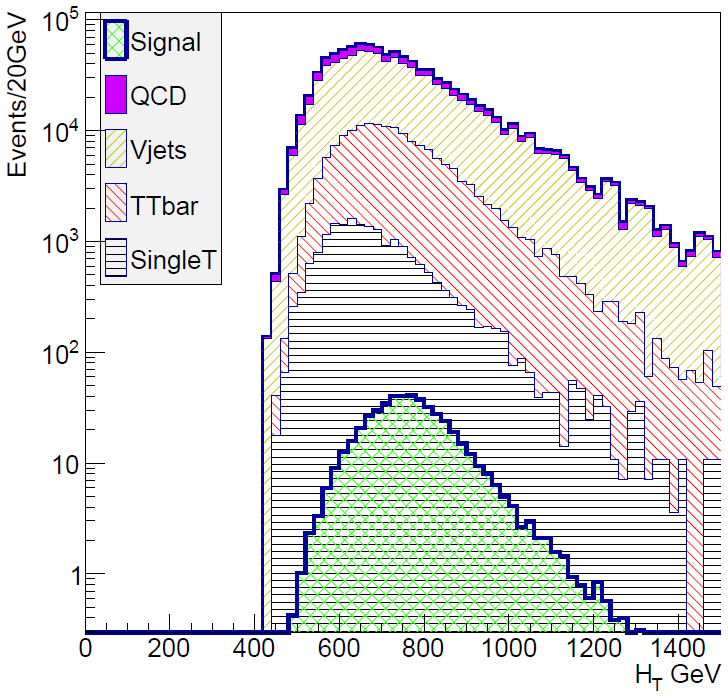
\includegraphics[width=0.8\textwidth]{figs/Ana/HT.png}
    \caption{Distribution of $H_{T}$ variable for data and the sum of the MC samples normalized to luminosity. The signal sample (M=700 \GeVcc) is over-imposed on top of the stack of the MC samples. The gray band represents the statistical uncertainties from the sum of the MC background. Reasonable agreement is observed, multijet process is the dominant process at this stage.}
    \label{fig:HT}
  \end{center}
\end{figure}

Finally the basic selection ends with the request of a minimum of b-tagged jets. CSV algorithm (described in section~\ref{sec:bid}) was used to identify jets coming from a b quark. We define b-tagged jets as jets that were b-tagged by CSV algorithm while b-jets as jets truly coming from a b-quark. The medium working point was chosen as it allows to have a high efficiency on b-jet identification with a low fake rate from c and light quarks and it allows to keep a high efficiency on signal. In the full hadronic final state, the T decays in three b-quarks, a \bbbar system coming from the Higgs and an additional b quark from the t-quark, and two light jet from the W boson produced by the top. Accordingly, one expects signal events to have at least 3 b-tagged jets, while \ttbar~events should have 2 and 0 for QCD, as mean values.

In principle we can use several working points to establish the b-tagged jets content of events. For example, one can require to have events with at least 3 b-tagged jets one with tight working point and two with medium working points. We have studied all possible combinations from the three available working points (loose (CSVL), medium (CSVM) and tight (CSVT)) to require at least 3 CSV b-tagged jets in order to establish which combination gave the best $S/B$ while keeping the most of signal events. For the study, we have used as signal the $M=700$ \GeVcc signal sample and as backgrounds \ttbar, QCD\_HT-500To1000 and QCD\_HT-1000ToInf MC samples. The study was performed up to \HT cut. The results of the study are contained in table~\ref{tab:BCutStudy}. From it, one can see that the most efficient cut to discriminate signal from backgrounds and to keep signal is to require at least 3 CSVM b-tagged jets. At this stage is extremely important to keep enough signal, because the next step of the analysis is T reconstruction.

\begin{table}[htbH]
\begin{center}
\resizebox{\textwidth}{!}{
\begin{tabular}{| c || c | c | c | c | c | c |}
\hline 
\textit{At least} & $\epsilon(S)$ [\%] & $\epsilon(t\bar{t})$ [\%] & $\epsilon(\text{QCD\_HT-500To1000})$ [\%] & $\epsilon(\text{QCD\_HT-1000ToInf})$ [\%] & $\frac{S}{B}\times 10^{3}$ & $\frac{S}{S+B}\times 10^{2}$ \\
\hline
3 CSVL            & $65 \pm 1$  & $38 \pm 0.07$  & $6 \pm 0.03$ & $7 \pm 0.03$             & $0.4 \pm 5\times 10^{-3}$  & $24.8 \pm 0.3$ \\
3 CSVM            & $31 \pm 1$  & $8 \pm 0.03$  & $1 \pm 0.01$ & $0.6 \pm 0.01$            & $1.8 \pm 5\times 10^{-2}$  & $38.2 \pm 0.8$ \\
1 CSVL and 2 CSVM & $70 \pm 1$  & $46 \pm 0.09$  & $5 \pm 0.03$ & $5 \pm 0.02$             & $0.5 \pm 7\times 10^{-3}$  & $30.3 \pm 0.4$ \\
2 CSVL and 1 CSVM & $89 \pm 1$  & $72 \pm 0.1$  & $14 \pm 0.05$ & $15 \pm 0.04$            & $0.2 \pm 3\times 10^{-3}$  & $23.3 \pm 0.2$  \\
2 CSVM and 1 CSVT & $64 \pm 1$  & $41 \pm 0.08$  & $4 \pm 0.02$ & $4 \pm 0.02$             & $0.6 \pm 8\times 10^{-3}$  & $31.1 \pm 0.4$  \\
1 CSVM and 2 CSVT & $39 \pm 1$  & $21 \pm 0.05$  & $2 \pm 0.01$ & $1 \pm 0.01$             & $0.7 \pm 1\times 10^{-2}$  & $27.5 \pm 0.4$  \\
3 CSVT            & $9 \pm 0.3$  & $1 \pm 0.01$  & $0.1 \pm 0.03$ & $0.09 \pm 0.002$       & $3.1 \pm 2\times 10^{-1}$  & $27.3 \pm 1.1$  \\
1 CSVL and 2 CSVT & $39 \pm 1$  & $21 \pm 0.05$  & $2 \pm 0.01$ & $1 \pm 0.01$             & $0.7 \pm 1\times 10^{-2}$  & $27.5 \pm 0.4$  \\
2 CSVL and 1 CSVT & $76 \pm 1$  & $59 \pm 0.1$  & $7 \pm 0.03$  & $7 \pm 0.03$             & $0.4 \pm 4\times 10^{-3}$  & $26.8 \pm 0.3$  \\
1 CSVL and 1 CSVM and 1 CSVT &  $80 \pm 1$ &  $69 \pm 0.1$ & $11 \pm 0.04$ & $11 \pm 0.04$ & $0.3 \pm 3\times 10^{-3}$  & $23.4 \pm 0.2$  \\
\hline

\hline
\end{tabular}
}
\caption{Comparative study of different possible combinations to require at least 3 b-tagged jets with CSVL, CSVM and CSVT working points. Efficiencies of cuts over signal and principal MC background samples are presented, as well as $\frac{S}{B}$ and $\frac{S}{S+B}$. We chose the cut giving highest $\frac{S}{S+B}$, at least 3CSVM. High values of $\frac{S}{S+B}$ point a good discrimination while keeping signal.\label{tab:BCutStudy}}
\end{center}
\end{table}

As described in section~\ref{sec:bid} b-tagging is performed using a complex procedure where several jet variables are taken into account. It strongly depends on the ability to find displaced vertices, reason why it has been restricted to jets in $\eta<=2.4$. As MC conditions are ideal in comparison with real data (less noise, perfect detector operation, etc.), b-tagging bring different results in data than in MC. Thus, a correction must be applied to MC to mimic b-tagging response on data. In general, CSV algorithm is slightly more efficient for b-tagging b-jets in MC than in data. Additionally, it also gives more fakes coming from light jets in data than in MC. To match MC to data a scale factor has been derived by the collaboration. It is defined for each jet depending on its flavor (b and c or light), \pt and $\eta$. In equation~\ref{eq:Sfs}, it can be found the functions defining the scale factors for CSVM working point. The functions are defined as $SF^{flavor}_{\eta}(p_{T})$.

\begin{eqnarray}
  \label{eq:Sfs}
  SF^{b\; or\; c}_{|\eta|\le 2.4}(x) & = & 0.938887 + 0.00017124x - 2.76366 \times 10^{-7}x^{2} \nonumber \\
  SF^{light}_{|\eta|\le 0.8}(x) & = & 1.07541 + 0.00231827x - 4.74249 \times 10^{-6}x^{2}  \nonumber \\
  &  & +2.70862 \times 10^{-9}x^{3} \nonumber \\
  SF^{light}_{0.8 < |\eta|\le 1.6}(x) & = & 1.05613 + 0.00114031x - 2.56066 \times 10^{-6}x^{2} \nonumber \\
  &  & + 1.67792 \times 10^{-9}x^{3} \nonumber \\
  SF^{light}_{1.6 < |\eta|\le 2.4}(x) & = & 1.05625 + 0.000487231x - 2.22792 \times 10^{-6}x^{2} \nonumber \\
  &  & + 1.70262 \times 10^{-9}x^{3}
\end{eqnarray}

In order to apply b-tagging scale factors to MC samples, a recommended methods by the collaboration was used. The chosen method allows to calculate a weight per events in terms of its jet flavor content. The weight definition can be found in equation~\ref{eq:SFW}, 

\begin{equation}
  \label{eq:SFW}
  w=\frac{P(\text{DATA})}{P(\text{MC})}
\end{equation}where

\begin{eqnarray}
  \label{eq:DataMCSFP}
  P(\text{MC}) & = & \prod_{i=\text{tagged}} \varepsilon_i \prod_{j=\text{not tagged}} (1-\varepsilon_j) \\
  P(\text{DATA}) & = & \prod_{i=\text{tagged}} \text{SF}_i \varepsilon_i \prod_{j=\text{not tagged}} (1-\text{SF}_j \varepsilon_j)
\end{eqnarray}the products are defined over all jets in the event. $\varepsilon$ represents the b-tagging efficiency. Efficiencies were calculated for each MC sample as function of flavor, \pt and $\eta$. In figure~\ref{fig:SignalBEff} it can be found CSVM b-tagging efficiencies for b, c and light jet flavors for signal MC sample. In figure~\ref{fig:ttbarBEff} and~\ref{fig:QCDBEff} can be found the same efficiencies for \ttbar and QCD MC samples. Also, the calculated weights for each MC are shown in figure~\ref{fig:SFweight}. 

\begin{figure}[!Hhtbp]
  \begin{center}
    \includegraphics[width=0.8\textwidth]{figs/Ana/SF_weight.png}
    \caption{Distribution of weight from b-tagging scale factors for all MC samples.}
    \label{fig:SFweight}
  \end{center}
\end{figure}

\begin{figure}[!Hhtbp]
  \begin{center}
    \includegraphics[width=0.8\textwidth, height=0.33\textheight]{figs/Ana/Signal_beff.png}
    \includegraphics[width=0.8\textwidth, height=0.33\textheight]{figs/Ana/Signal_ceff.png}
    \includegraphics[width=0.8\textwidth, height=0.33\textheight]{figs/Ana/Signal_leff.png}
    \caption{CSVM b-tagging efficiency for b-jets [left], c-jets [center] and light jets [right] as function of \pt and $\eta$ for signal.}
    \label{fig:SignalBEff}
  \end{center}
\end{figure}

\begin{figure}[!Hhtbp]
  \begin{center}
    \includegraphics[width=0.8\textwidth, height=0.33\textheight]{figs/Ana/ttbar_beff.png}
    \includegraphics[width=0.8\textwidth, height=0.33\textheight]{figs/Ana/ttbar_ceff.png}
    \includegraphics[width=0.8\textwidth, height=0.33\textheight]{figs/Ana/ttbar_leff.png}
    \caption{CSVM b-tagging efficiency for b-jets [left], c-jets [center] and light jets [right] as function of \pt and $\eta$ for \ttbar.}
    \label{fig:ttbarBEff}
  \end{center}
\end{figure}

\begin{figure}[!Hhtbp]
  \begin{center}
    \includegraphics[width=0.8\textwidth, height=0.33\textheight]{figs/Ana/QCDHT500_beff.png}
    \includegraphics[width=0.8\textwidth, height=0.33\textheight]{figs/Ana/QCDHT500_ceff.png}
    \includegraphics[width=0.8\textwidth, height=0.33\textheight]{figs/Ana/QCDHT500_leff.png}
    \caption{CSVM b-tagging efficiency for b-jets [left], c-jets [center] and light jets [right] as function of \pt and $\eta$ for QCD\_HT-500To1000.}
    \label{fig:QCDBEff}
  \end{center}
\end{figure}

Efficiencies were calculated using the following formula:

\begin{equation}
  \label{eq:btaggingeff}
  \varepsilon_f(i,j) = \frac{N_f^\text{b-tagged}(i,j)}{N_f^\text{Total}(i,j)}
\end{equation} where $ N_f^\text{Total}(i,j) $ and $ N_f^\text{b-tagged}(i,j) $ are the total number and the number of b-tagged jets, respectively, of flavor $ f $ in the $ (p_\text{T},\eta) $ bin $ (i,j) $. The determination of jet flavor is done via the matching of jets to quarks from parton level simulation. The matching is not always successful and some jets can have no parton matched, i.e. no associated flavor. These jets, as well as jets coming from gluons, were included in light flavor category, following official recommendations.

Finally, data was compared to MC predictions in figure~\ref{fig:Nb} in the number of CSVM b-tagged jets. The different data/MC comparisons presented are used for illustration and to check that pileup and b-tagging corrections in MC are correctly applied. For final analysis results only signal MC samples are used, as backgrounds were estimated from data.

\begin{figure}[!Hhtbp]
  \begin{center}
    \includegraphics[width=0.8\textwidth]{figs/Ana/NCSVM.png}
    \caption{B-tagged CSVM jet multiplicity for data and MC samples before requiring at least 3 CSVM b-tagged jets. This criteria is the last criteria definition the basic selection. The sum of MC is normalized to the integrated luminosity in the data.}
    \label{fig:Nb}
  \end{center}
\end{figure}
%\begin{TOINCLUDE}Plots of pt and eta of six leading jets, number of vertices, HT and number of CSVM b-tagged jets\end{TOINCLUDE}

\subsection{T reconstruction with a $\chi^{2}$ sorting algorithm}
\label{sec:chi2}

A crucial step to reconstruct T mass is to identify correctly the five jets produced by it. Events passing basic selection have at least 6 jets, but jet multiplicity can be much greater. In consequence, the process of identifying T-jets is not trivial. 

A $\chi^{2}$ sorting algorithm has been used to identify the T decay products and to reconstruct the Higgs and top. This technique is based in the definition of a variable constructed from the information of objects under consideration and the properties of the particles to be reconstructed. The variable is computed for all possible object combinations. The best the fit of the chosen objects to the required reconstruction, minimal is the value of the variable. An example of this method can be found in~\cite{Brochet:1956723}. 

We define the $\chi^{2}$ variable in equation~\ref{eq:chi2def}. The values used as inputs were: $M_{H}=125$~\GeVcc, $M_{W}=84.06$~\GeVcc, $M_{t}=175.16$~\GeVcc, $\sigma_{H}=12.4$~\GeVcc (from~\cite{Chatrchyan:2013zna}), and $\sigma_{W}=10.12$~\GeVcc and $\sigma_{t}=17.35$~\GeVcc (from~\cite{Brochet:1956723}). For the Higgs reconstruction only CSVM b-tagged jets are considered. For W reconstruction all jets with a \ptg{30} were considered. And for the top reconstruction one b-tagged jet and the pair of jets used for the W. B-tagging status of jets used for the W was not used.

\begin{equation}
\chi^{2}=\frac{(M_{H}-M_{bb})^{2}}{\sigma_{H}^{2}}+\frac{(M_{W}-M_{jj})^{2}}{\sigma_{W}^{2}}+\frac{(M_{t}-M_{bjj})^{2}}{\sigma_{t}^{2}}
\label{eq:chi2def}
\end{equation}

One can evaluate the efficiency of the reconstruction of each resonance (Higgs, W, top and T) using each MC signal sample. We define two efficiencies, the exclusive efficiency that is the ratio between the number of events where the particle was well reconstructed and the number of events where all jets where correctly matched to a parton, and the inclusive efficiency where the ratio is done with respect to the total number of events. Both efficiencies were evaluated after basic selection. The efficiency values are found, for all MC signal samples, in figure~\ref{fig:RecEff}. We found an exclusive efficiency of around 70\% for the T independently of the MC signal sample.

\begin{figure}[!Hhtbp]
  \begin{center}
    \includegraphics[width=0.46\textwidth]{figs/Ana/Exclusive_Efficiency_V8.png}
    \includegraphics[width=0.46\textwidth]{figs/Ana/Inclusive_Efficiency_V8.png}
    \caption{Reconstruction efficiency taking into account only events where jets could be matched to partons [left] and to total number of events [right]}
    \label{fig:RecEff}
  \end{center}
\end{figure}

In figure~\ref{fig:WHt} it can be found the reconstructed W, Higgs and top masses by the $\chi^{2}$ sorting algorithm. Additionally, in figure~\ref{fig:RecT} are shown the reconstructed T mass for all used MC signal samples. Finally, in table~\ref{tab:SignalWidths} are presented the results from fitting with a gaussian all mass points after full selection. The found widths for T mass varies between 30 to 50 \GeVcc, what means 6\% of T mass. This fit is used to calculate the expected yields for the signal for calculation of limits.

\begin{figure}[!Hhtbp]
  \begin{center}
    \includegraphics[width=0.32\textwidth]{figs/Ana/TopMass_S700.png}
    \includegraphics[width=0.32\textwidth]{figs/Ana/WMass_S700.png}
    \includegraphics[width=0.32\textwidth]{figs/Ana/HiggsMass_S700.png}
    \caption{Reconstructed top, W and H for the T mass point of 700 \GeVcc}
    \label{fig:WHt}
  \end{center}
\end{figure}

\begin{figure}[!Hhtbp]
  \begin{center}
    \includegraphics[width=0.45\textwidth]{figs/Ana/HundresdsMassChi2Tp.png}
    \includegraphics[width=0.45\textwidth]{figs/Ana/FiftiesMassChi2Tp.png}
    \caption{Reconstructed T mass for all mass points from $chi^{2}$ sorting algorithm.}
    \label{fig:RecT}
  \end{center}
\end{figure}

\begin{table*}[htbH]
\begin{center}
\begin{tabular}{|c|c|c|c|c|}
\hline 
\multicolumn{2}{|c}{Generated} & \multicolumn{3}{|c|}{Reconstructed} \\
Mass (GeV/$c^{2}$) & Width (GeV/$c^{2}$) & Mass (GeV/$c^{2}$) & Width (GeV/$c^{2}$) & $\chi^{2} /$ndf\\
\hline
600 & 0.62 &$604.60\pm14.18$ & $32.44\pm10.37$ & 4.99/4\\
650 & 0.80 &$644.56\pm12.64$ & $35.53\pm9.54$ & 8.03/4\\
700 & 1.02 &$691.79\pm13.65$ & $41.16\pm9.75$ & 10.80/7\\
750 & 1.27 &$736.26\pm15.53$ & $45.38\pm11.46$ & 10.24/7\\
800 & 1.56 &$782.97\pm18.12$ & $49.35\pm13.49$ & 23.67/7\\
850 & 1.89 &$832.49\pm17.92$ & $47.39\pm13.28$ & 15.71/7\\
900 & 2.26 &$881.38\pm19.13$ & $45.58\pm14.24$ & 11.01/7\\
950 & 2.67 &$929.02\pm25.02$ & $51.54\pm18.96$ & 14.54/7\\
1000 & 3.13 &$970.36\pm32.18$ & $53.34\pm25.14$ & 11.51/7\\
\hline
\end{tabular}
\caption{Reconstructed mass and width for T candidate after full analysis selection from a gaussian fit for each signal mass generated. \label{tab:SignalWidths}}
\end{center}
\end{table*}

The $\chi^{2}$ distribution is plotted in figure~\ref{fig:chi2}. Signal events have preferentially a $\chi^{2}<50$, while multijet and \ttbar backgrounds have much longer tail for high $\chi^{2}$ values.

\begin{figure}[!Hhtbp]
  \begin{center}
    \includegraphics[width=0.8\textwidth]{figs/Ana/chi2Nm1.png}
    \caption{Distribution of $\chi^{2}$ variable for data and MC samples. The signal sample used has a T mass of 700 \GeVcc. Backgrounds present higher values than signal.}
    \label{fig:chi2}
  \end{center}
\end{figure}
%\begin{TOINCLUDE}Table with inclusive and exclusive reconstruction efficiency. Plots of mass of reconstructed T, W, H and top right after reconstruction for all mass points. Table with gaussian fit results.\end{TOINCLUDE}

\subsection{Selection based on reconstructed objects}

After the reconstruction procedure, a final step in the selection is performed based on the properties of reconstructed objects. This last set of cuts we have optimized to obtain the highest discrimination between signal and backgrounds. The discrimination of the selection has been evaluated from the estimator $S/B$, where we have used as signal the $M(T)=700$ \GeVcc MC sample, and \ttbar and QCD\_HT-500To1000 for the backgrounds. Moreover, as we pretend to do a reconstruction of T mass we need to keep a considerable number of events at the end of the selection, we have restricted the selection to keep at least 10 signal events. 

The principal limitation for the optimization of the selection is the lack of statistics in the multijet MC sample. Reason why, we preferred the selection that killed completely QCD\_HT-500To1000 MC sample, and gave us the highest $S/B$ value. MC samples for backgrounds were used only for selection optimization and illustration in the data versus MC plots. The limit setting and final results were produced with an estimation of backgrounds performed from data.  

The first variable considered for selection is the $\chi^{2}$. As seen in figure~\ref{fig:chi2}, signal tends to have smaller values of $\chi^{2}$ than backgrounds. In figure~\ref{fig:chi2cut} it can be seen a scan of the efficiency of cutting on the $\chi^{2}$ for the values displayed in the x-axis. These efficiencies were evaluated for the signal ($M(T)=700$ \GeVcc), \ttbar and QCD\_HT-500To1000 MC samples. In addition, it can be seen the ratio of the efficiency of signal over the efficiency of the cut on \ttbar and QCD samples, this ratios are directly proportional to $S/B$. One can see from the figure. In agreement with the increase of $S/B$ as measure of the cut value, we have chosen to cut on $\chi^{2}<8$. One additional feature of this cut, that will be seen in section~\ref{sec:bkg}, is that this cut ensures the agreement of the control sample with the signal sample for the background estimation. 

\begin{figure}[!Hhtbp]
  \begin{center}
    \includegraphics[width=0.8\textwidth]{figs/Ana/chi2_SoB.png}
    \caption{Efficiency of cutting on $chi^{2}<x$ as function of cut value for $M=700$ \GeVcc signal sample, \ttbar and QCD\_HT-500To1000 MC samples. Ratios between efficiency for signal and each background are also displayed.}
    \label{fig:chi2cut}
  \end{center}
\end{figure}

After cutting in $\chi^{2}$, events were required to have the two b-quarks used to reconstruct the Higgs to have $\Delta R(bb)<1.2$. In figure~\ref{fig:DRbb} it can be seen the comparison between data and MC for $\Delta R(bb)$ before cutting on it. It is also shown an equivalent cut efficiency study as for $\chi^{2}$ variable. 

\begin{figure}[!Hhtbp]
  \begin{center}
    \includegraphics[width=0.45\textwidth]{figs/Ana/DRbb_SoB.png}
    \includegraphics[width=0.45\textwidth]{figs/Ana/DRbbNm1.png}
    \caption{Efficiency of cutting on $\Delta R(bb)<x$ as function of cut value for $M=700$ \GeVcc signal sample, \ttbar and QCD\_HT-500To1000 MC samples and ratios between efficiency for signal and each background [left]. $\Delta R$ of the 2 b-tagged jets used to reconstruct the Higgs candidate after basic selection [right]. The signal which is simply overlaid prefers low $\Delta R$ while backgrounds have larger distribution at higher value. The gray band represents the statistical uncertainties from the sum of the MC background.}
    \label{fig:DRbb}
  \end{center}
\end{figure}

Afterward, events were required to have a reconstructed W and H with a $1.6<\Delta R (W_{cand} H_{cand})<4.0$. This variable presents a peak for signal at 2.8, as it can be seen in figure~\ref{fig:DRWH}. Backgrounds also have a peak around 3, but have larger tails than signal. The cut then has been chosen to keep events inside a window of 1.2 around the peak. In the same figure it can be seen the cut efficiency plot for this variable for different window values.

\begin{figure}[!Hhtbp]
  \begin{center}
    \includegraphics[width=0.45\textwidth]{figs/Ana/DRWH_SoB.png}
    \includegraphics[width=0.45\textwidth]{figs/Ana/DRWHNm1.png}
    \caption{Efficiency of cutting on $|\Delta R(W_{cand} H_{cand})-2.8|<x$ as function of cut value for $M=700$ \GeVcc signal sample, \ttbar and QCD\_HT-500To1000 MC samples and ratios between efficiency for signal and each background [left]. Distribution for $\Delta R (W_{cand} H_{cand})$ for data and the sum of Monte Carlo samples [right]. All others criteria are applied up to this one.}
    \label{fig:DRWH}
  \end{center}
\end{figure}

One important difference between signal and backgrounds, is that in signal events there is a real Higgs decaying into \bbbar. Thus, a resonance peak is expected to appear for the \bbbar system for signal events, while it is not the case for backgrounds. In consequence, events were required to have a Higgs candidate mass between 105 and 145 \GeVcc. Efficiency plot of cutting on events outside a window around 125 \GeVcc in the Higgs candidate mass is shown in figure~\ref{fig:HiggsMassDMC}. In the same figure the Higgs candidate mass is shown before cutting on it, for data and MC samples.

\begin{figure}[!Hhtbp]
  \begin{center}
    \includegraphics[width=0.45\textwidth]{figs/Ana/HM_SoB.png}
    \includegraphics[width=0.45\textwidth]{figs/Ana/HMNm1.png}
    \caption{Efficiency of cutting on $|M(H_{cand})-125|<x$ as function of cut value for $M=700$ \GeVcc signal sample, \ttbar and QCD\_HT-500To1000 MC samples and ratios between efficiency for signal and each background [left]. Distribution for $M(H_{cand})$ for data and the sum of Monte Carlo samples [right]. All others criteria are applied up to this one.}
    \label{fig:HiggsMassDMC}
  \end{center}
\end{figure}

At this stage of the selection we have found a pair of variables to focus in suppress \ttbar background. However QCD is comparable to \ttbar, it is this second background the most similar to our signal due to the presence of a real top. in addition, the \ttbar system is capable to fake a Higgs with similar properties than the one in signal events. To identify how the \ttbar system was making Higgs fakes we have explored from MC truth information the quarks that were chosen by $\chi^{2}$ sorting algorithm as coming form the Higgs. In figure~\ref{fig:RecohiggsMCTruth} it can be seen the Higgs reconstruction cases, coded as follows:

\begin{itemize}
\item Bin 0: Higgs candidate reconstructed from two b-quarks coming each one from a top quark.
\item Bin 1: Higgs candidate reconstructed from Higgs \bbbar system.
\item Bin 2: Higgs candidate reconstructed from one quark from the Higgs and one b-quark from a top.
\item Bin 3: Higgs candidate reconstructed from one quark from the Higgs and one quark from a W.
\item Bin 4: Higgs candidate reconstructed from one b-quark from the top and one quark from a W.
\item Bin 5: Higgs candidate reconstructed from two quarks coming from W bosons.
\item Bin 6: Higgs candidate reconstructed from one jet from the Higgs and one additional quark (not from Higgs, W nor top).
\item Bin 7: Higgs candidate reconstructed from one b-quark from a top and one additional quark (not from Higgs, W nor top).
\item Bin 8: Higgs candidate reconstructed from one jet from a W and one additional quark (not from Higgs, W nor top).
\item Bin 9: Higgs candidate reconstructed from two additional quarks (not from Higgs, W nor top).
\end{itemize}

\begin{figure}[!Hhtbp]
  \begin{center}
    \includegraphics[width=0.45\textwidth]{figs/Ana/HiggsRecoMCTruth_S700.png}
    \includegraphics[width=0.45\textwidth]{figs/Ana/HiggsRecoMCTruth_TTJets.png}
    \caption{Higgs candidate reconstruction MC truth for signal (M=700 \GeVcc) [left] and \ttbar [right] MC samples. in signal the Higgs is reconstructed preferentially from two jets coming from the Higgs (bin 1) while for \ttbar the Higgs candidate is reconstructed preferentially from a b-quark from a top and a quark from a W boson (bin 4).}
    \label{fig:RecohiggsMCTruth}
  \end{center}
\end{figure}

In this figure one can sees that the Higgs candidate is preferentially reconstructed in \ttbar events from a b-quark coming from a top and one quark coming from a W boson. As one top is also reconstructed, this means that the Higgs is being reconstructed from the second top. Thus, to identify \ttbar events one can try to reconstruct the second top from the b-tagged jets used for the Higgs and one additional jet not used by $\chi^{2}$ algorithm. As this extra jet is coming from a top we expect it to be quite boosted, then we reconstruct the second top from the two Higgs jets and the leading jet not used by the $\chi^{2}$ algorithm. We also define a second top from the sub-leading Higgs jet and leading jet not used by the $\chi^{2}$ algorithm. The distribution for the second top mass can be seen in figure~\ref{fig:2ndTM} for data and MC samples. It shows a clear peak at the top mass value for \ttbar events.

\begin{figure}[!Hhtbp]
  \begin{center}
    \includegraphics[width=0.45\textwidth]{figs/Ana/M2ndTopNm1.png}
    \caption{Second top mass distribution for data and the sum of the Monte Carlo samples. Selection criteria applied up to Higgs mass cut.}
    \label{fig:2ndTM}
  \end{center}
\end{figure}

We have build a variable with the second top and second W boson to discriminate signal from background (mainly \ttbar). To increase the separation between backgrounds and signal we don't take only the second top mass, but we add the the second W boson mass and divide by the Higgs mass. The distribution for this variables is shown in figure~\ref{fig:m2thp} for data and the sum of MC samples. Events with $(M(top^{2nd})+M(W^{2nd}))/M(H)>6.8$ were selected.

\begin{figure}[!Hhtbp]
  \begin{center}
    \includegraphics[width=0.45\textwidth]{figs/Ana/M2HP_SoB.png}
    \includegraphics[width=0.45\textwidth]{figs/Ana/M2HPNm1.png}
    \caption{Efficiency of cutting on $(M(top^{2nd})+M(W^{2nd}))/M(H)>x$ as function of cut value for $M=700$ \GeVcc signal sample, \ttbar and QCD\_HT-500To1000 MC samples and ratios between efficiency for signal and each background [left]. Distribution of $(M(top^{2nd})+M(W^{2nd}))/M(H)$ for data and the sum of the Monte Carlo samples [right]. All others criteria are applied before this one. The low statistics in the multijet (QCD) MC sample is visible at this stage. The gray band represents the statistical uncertainties from the sum of the MC background and it is dominated by QCD samples.}
    \label{fig:m2thp}
  \end{center}
\end{figure}

The selection continues taking advantage of the angular relation between the T and the quark produced in association with it for signal events. We know that they are produced preferentially with high $\Delta R$ while for backgrounds the two objects have lower $\Delta R$. We identify with the leading jet not used by the reconstruction procedure with the jet produced with the T. We call this jet the 6th jet, $j^{6}$. The distribution of $\Delta R (T j^{6th})$, before cutting on it, can be found in figure~\ref{fig:jet6} for data and MC samples along with the efficiency plot of cutting on $\Delta R (T j^{6th})$ for $M=700$ \GeVcc signal sample, \ttbar and QCD\_HT-500To1000 MC samples. At this stage the statistics in QCD MC samples begin to be very low. We select events that have $\Delta R (T j^{6th})>4.8$. 

\begin{figure}[!Hhtbp]
  \begin{center}
    \includegraphics[width=0.45\textwidth]{figs/Ana/DRTp6thJ_SoB.png}
    \includegraphics[width=0.45\textwidth]{figs/Ana/DRTp6JNm1.png}
    \caption{Efficiency of cutting on $\Delta R (T j^{6th})>x$ as function of cut value for $M=700$ \GeVcc signal sample, \ttbar and QCD\_HT-500To1000 MC samples and ratios between efficiency for signal and each background [left]. Distributions for $\Delta R (T j^{6th})$  for data and the sum of Monte Carlo samples [right]. All others criteria are applied up to this one. The low statistics in the multijet (QCD) MC sample is visible at this stage. The gray band represents the statistical uncertainties from the sum of the MC background and it is dominated by QCD samples.}
    \label{fig:jet6}
  \end{center}
\end{figure}

For the last cut we define the \textit{Relative} $H_{T}$ as the sum of the \pt of the Higgs candidate plus the \pt of the top candidate divided by $H_{T}$ of the event. This variable measures how much \pt of the event is coming from the Higgs and top candidates. As for signal events the top and Higgs candidates are coming from a highly massive object, that is decaying into these two objects, we expect signal events to have a relative $H_{T}$ closer to 1 than backgrounds events. The relative $H_{T}$ distribution can be found in figure~\ref{fig:RelHtMass} for data and the sum of MC samples before cutting on it, with the rest of the selection applied. At this stage the QCD MC samples have very low statistics. In the same figure can be found the efficiency plot of the cut. We keep events that have a Relative $H_{T}>0.67$. 

\begin{figure}[!Hhtbp]
  \begin{center}
    \includegraphics[width=0.45\textwidth]{figs/Ana/RelHT_SoB.png}
    \includegraphics[width=0.45\textwidth]{figs/Ana/RelHTNm1.png}
    \caption{Efficiency of cutting on Relative $H_{T}>x$ as function of cut value for $M=700$ \GeVcc signal sample, \ttbar and QCD\_HT-500To1000 MC samples and ratios between efficiency for signal and each background [left]. Distribution of Relative $H_{T}$ for data and the sum of the Monte Carlo samples [right]. All others criteria are applied up to this one. At this stage multijet (QCD) MC sample have very low statistics. The gray band represents the statistical uncertainties from the sum of the MC background and it is dominated by QCD samples.}
    \label{fig:RelHtMass}
  \end{center}
\end{figure}

To check the progression of the selection, in table~\ref{tab:Estimators} is shown the $S/B$ after each cut after the reconstruction of objects. In the table we can see an increase of the estimator at each step, which means that with each cut the discrimination between signal and background increments. For this calculation $M=700$ \GeVcc signal, \ttbar and QCD\_HT-500To1000 MC samples were used. %As QCD statistics decrease rapidly, and at some point they are very low, we calculate the estimator with respect to \ttbar and QCD samples separately.

\begin{table}[htbH]
\label{tab:Estimators}
\begin{center}
%\resizebox{\textwidth}{!}{
\begin{tabular}{|c|c|c|}
\hline 
Cut & $S/B$ & $S/\sqrt{S+B}$ \\
\hline
$\chi^{2}<8$ & $3.4\ex{-2} \pm 2.85\ex{-3}$  & $ 0.96 \pm 0.05$  \\
$\Delta R(bb)<1.2$ & $4.76\ex{-2} \pm 4.52\ex{-3}$ & $1.10 \pm 0.07$  \\
$1.6<\Delta R (W_{cand} H_{cand})<4.0$ & $4.82\ex{-2} \pm 4.59\ex{-3}$  & $1.10 \pm 0.07$  \\
$105$ \GeVcc $< M(H_{cand}) < 145$ \GeVcc & $6.38\ex{-2} \pm 6.81\ex{-3}$  & $1.21 \pm 0.08$  \\
$(M(top^{2nd})+M(W^{2nd}))/M(H_{cand})>6.8$ & $0.15 \pm 0.03$  & $1.45 \pm 0.17$  \\
$\Delta R (T j^{6th})>4.8$ & $0.42 \pm 0.19$  & $1.66 \pm 0.32$  \\
Relative $H_{T}>0.67$ & $1.16 \pm 0.17$  & $2.13 \pm 0.17$  \\
\hline
\end{tabular}
\caption{$S/B$ and $S/\sqrt{S+B}$ from MC samples for each step of the selection after reconstruction. Only $M=700$ \GeVcc signal, \ttbar and QCD\_HT-500To1000 MC samples were used.}
%}
\end{center}
\end{table}
%\begin{TOINCLUDE}$N-1$ plots for object selection variables. Table with $S/B$ and $S/\sqrt{S+B}$ from MC for each step of the selection. \end{TOINCLUDE}

\subsection{Efficiencies}
\label{sec:eff}

\subsubsection{Trigger}
\label{sec:trigger_ana}

We have computed the trigger efficiency using as reference the prescaled trigger HLT\_HT400\_v*. From other analyses using $H_{T}$ triggers, as in~\cite{Khachatryan:2015axa}, around 100 GeV additional cut on top of trigger cut, are needed to reach the trigger plateau. Assuming it is the case also for HLT\_HT400\_v*, the cut on the selection requiring $H_{T}>550$ GeV should select events in the efficiency plateau. Trigger efficiency is normally evaluated after full selection. However, as HLT\_HT400 leaving very small amount of events after full selection, we have decided to compute the trigger efficiency at various earlier selection stages. Additionally, instead of calculating a scale factor to match trigger efficiency in MC samples to data we have studied the differences to assign an overall systematic effect. 

We have used the \pt of the 6th leading jet to parametrize trigger efficiency. This efficiency is defined as the ratio between the number of events passing both triggers (HLT\_HT400 and HLT\_Dijet80\_Dijet60\_Dijet20) and the number of events passing only HLT\_HT400. HLT\_HT400 is used as unbiased sample with respect to HLT\_Dijet80\_Dijet60\_Dijet20. In figure~\ref{fig:TrigEff} it can be seen the trigger efficiency as function of 6th leading jet \pt after $chi^{2}$ cut for all signal MC samples. 

\begin{figure}[!Hhtbp]
  \begin{center}
    \includegraphics[width=0.45\textwidth]{figs/Ana/Trigger_Eff_hundreds_chi2.png}
    \includegraphics[width=0.45\textwidth]{figs/Ana/Trigger_Eff_fifties_chi2.png}
    \caption{Efficiency in data and the MC signal samples for events passing trigger bit HLT\_Dijet80\_Dijet60\_Dijet20 with respect to trigger bit HLT\_HT400 after standard selection up to $chi^{2}$ cut [included]. In the middle stage of the selection, we observe discrepancies between 10\% and 6\% at higher $p_{T}$. This efficiency is parametrized as function of the 6$^{th}$ jet $p_{T}$.}
    \label{fig:TrigEff}
  \end{center}
\end{figure}

The same efficiencies were additionally computed after cutting on the Higgs mass candidate. They can be found in figure~\ref{fig:TrigEffPostMH}. From them, we can see that MC signal samples are systematically underestimated by the trigger. This means that MC simulation of HLT applied to MC signal samples is cutting harder than in data. The observed differences vary between 10\% for low \pt and 5-6\% for high \pt.

\begin{figure}[!Hhtbp]
  \begin{center}
    \includegraphics[width=0.45\textwidth]{figs/Ana/Trigger_Eff_hundreds_HM.png}
    \includegraphics[width=0.45\textwidth]{figs/Ana/Trigger_Eff_fifties_HM.png}
    \caption{Efficiency in data and the MC signal samples for events passing trigger bit HLT\_Dijet80\_Dijet60\_Dijet20 with respect to trigger bit HLT\_HT400 after standard selection up to the Higgs-candidate mass selection. This efficiency is parametrized as function of the 6$^{th}$ jet $p_{T}$. The dispersion observed is mainly 6\%.}
    \label{fig:TrigEffPostMH}
  \end{center}
\end{figure}
%\begin{TOINCLUDE}Trigger efficiency plots\end{TOINCLUDE}

\subsubsection{Selection}
\label{sec:seleff}

In figure~\ref{fig:MPEff} it can be seen the total efficiency of the selection for each mass point MC sample. The lowest efficiency is for 600 \GeVcc mass point, around 1\%, while the highest is for 850 \GeVcc mass point, around 2\%. This efficiency has been calculated with respect to events passing trigger selection.  

\begin{figure}[!Hhtbp]
  \begin{center}
    \includegraphics[width=0.6\textwidth]{figs/Ana/Selection_Efficiency_V8.png}
    \caption{Selection efficiency for each mass point MC sample. Highest efficiency is achieved for 850 \GeVcc mass point.}
    \label{fig:MPEff}
  \end{center}
\end{figure}

%Additionally in table~\ref{tab:cutflow} we quote the efficiencies of each step of the selection for M=700 \GeVcc signal sample, multijet background, top background (\ttbar + single top), and diboson background MC samples. These efficiencies have calculated with respect to the number of events passing the trigger.

\begin{table*}[htbH]
\begin{center}
\resizebox{\textwidth}{!}{
\begin{tabular}{|c|c|c|c|c|c|}
\hline 
Selection & Cut & Signal (M=700 GeV/$c^{2}$) & Multijet & $t\bar{t}$ + single top & Diboson \\
\hline
\multirow{4}{*}{\rotatebox{90}{Basic}} & Trigger cut and $p_{T}$,$\eta$ selection & 52.68 & 18.53 & 36.55 & 16.14 \\
&$j^{1}>150$~GeV/c & 47.94 & 14.04 & 24.73 & 11.58 \\
&$H_{T}>550$~GeV/c & 47.65 & 13.53 & 24.22 & 11.16 \\
&$n_{b}^{CSVM}>=3$ & 14.57 & 0.06 & 1.98 & 0.15 \\
\hline
\multirow{10}{*}{\rotatebox{90}{Analysis}} & $\chi^{2}<8$ & 7.09 & $5\ex{-3}$ & 0.64 & 0.01  \\
&$\Delta R(bb) <1.2$ & 6.47 & $2\ex{-3}$ & 0.26 & $7\ex{-3}$ \\
&$1.6 < \Delta R (W_{cand} H_{cand}) < 4.0$ & 6.36 & $2\ex{-3}$ & 0.23 & $5\ex{-3}$ \\
&$105~\text{GeV}/c^{2} <M(H_{cand})<145~\text{GeV}/c^{2}$ & 5.65 & $1\ex{-3}$ & 0.17 & $2\ex{-3}$  \\
&$\frac{M(top^{2nd}_{cand})+M(W^{2nd}_{cand})}{M(H_{cand})}>6.8$ & 3.57 & $4\ex{-4}$ & 0.05 & $4\ex{-4}$ \\
&$ \Delta R (T' j^{6})>4.8$ & 2.01 & $2\ex{-5}$ & $6\ex{-3}$ & ---  \\
&$\frac{p_{T}(H_{cand})+p_{T}(top_{cand})}{H_{T}} > 0.67 $ & 1.79 & $4\ex{-7}$ & $3\ex{-3}$ & --- \\
\hline
\end{tabular}
}
\caption{Cumulative efficiencies, in \%, for signal and main background as a function of cuts applied. After $ \Delta R (T' j^{6})>4.8$ cut there are no longer events in the diboson MC samples. \label{tab:cutflow}}
\end{center}
\end{table*}
%\begin{TOINCLUDE}Table with efficiencies of full selection. Plot with selection efficiency for all mass points.\end{TOINCLUDE}

\section{Background estimation from data}
\label{sec:bkg}

As seen in latest sections, we don't count with enough statistics in background MC samples to estimate after full selection the expected contribution from SM backgrounds. Moreover, even in the case of having enough statistics the prediction from MC samples might not be reliable. According to this limitations, we needed to estimate our backgrounds from data.  

The main difficulty to estimate our backgrounds is the correlation between the variables used in the selection. This made impracticable traditional data driven background estimation methods as ABCD method (See for example~\cite{Khachatryan:2015axa}). Another difficulty was to derive to have a method that let us derive both principal backgrounds after full selection: multijets and \ttbar. Despite of this difficulties we have developed a method to derive from data the shape of backgrounds after full selection, and one additional method to estimate the normalization.

%\subsection{Known difficulties and tried methods}
%\label{sec:tried}
%
%Brief description of tried methods. One paragraph for matrix method one paragraph for tight-loose method.
%
%\begin{figure}[!Hhtbp]
%  \begin{center}
%    \includegraphics[width=0.3\textwidth]{figs/CMSlogo.png}
%    \caption{$p_{T}(H)$ and $p_{T}(top)$ correlation for backgrounds [left] and signal [right].}
%    \label{fig:HptTpt}
%  \end{center}
%\end{figure}\clearpage
%
%\begin{TOINCLUDE}2D plot of pT(H) and pT(top) to show correlation and table with ttbar+QCD and signal content in each region from ABCD method based on pT(H) and pT(top) \end{TOINCLUDE}

\subsection{Method for shape estimation}
\label{sec:bkgmet}

For the estimation of the shape of backgrounds we need to build a control region enriched by backgrounds while depleted in signal events. From the selection applied, the strongest cut to take out background events is $n_{b}^{CSVM}>=3$ (see table~\ref{tab:cutflow}). Reason why we take the number of b-tagged jets as variable to be loosen to obtain our control sample. 

We define the control region by events with the same selection as before but $n_{b}^{CSVL}>=3$ and vetoing events with $n_{b}^{CSVM}>=3$. With the veto on events with at least 3 CSVM b-tagged jets we prevent a high contamination from signal events in the control region. The control region then is basically formed of background events, mainly QCD and \ttbar. In figure~\ref{fig:CSSSSche} a schematic diagram for the construction of control and signal sample is presented.

\begin{figure}[!Hhtbp]
  \begin{center}
    \includegraphics[width=0.3\textwidth]{figs/Ana/SchematicControlSample.png}
    \caption{Schematic representation of signal and control sample. The big blue circle represents the ensemble of events with at least 3 CSVL b-tagged jets. The green circle represents the signal events while the circle filled with horizontal lines represents the signal sample (events with at least 3 CSVM b-tagged jets). The control sample then is the blue circle minus the horizontal line filled circle.}
    \label{fig:CSSSSche}
  \end{center}
\end{figure}

From this control sample we want then to estimate the background shape in the signal sample in the five jets invariant mass. Then the hypothesis is that the $M(5j)$ is equivalent in both control and signal sample, without any possible signal contribution. In the next section we will describe the procedure to test the validity of this hypothesis. 

\subsubsection{Validation}
\label{sec:validation}

In order to validate that the $M(5j)$ shape in the control sample can be used to estimate the background shape in the signal sample, we perform a shape comparison between both samples at different stages of the selection. An agreement of shapes is then shown at several stages between both samples. From this validation we also estimate a source of systematic uncertainty. The comparison is only performed in the $M(5j)$ range between 550 and 1100 \GeVcc, the range of explored signal masses.

The validation is performed at 4 different stages of the selection. Data in the control sample is compared to data in the signal sample. Also, even if MC statistics are poor to drive a conclusion for the validation procedure, we show the comparison for \ttbar sample (with good statistics), QCD samples (with poor statistics) and with full sum of MC samples. From the full set of comparison we can conclude if both shapes are in agreement or not. The 4 selected stages for the comparison are:
\begin{itemize}
\item Stage A: Selection up to $\chi^{2}<8$, included.
\item Stage B: Selection up to $1.6<\Delta R (W_{cand} H_{cand})<4.0$, included.
\item Stage C: Selection up to $\frac{M(top^{2nd}_{cand})+M(W^{2nd}_{cand})}{M(H_{cand})}>6.8$, included.
\item Stage D: Full selection.
\end{itemize}

As we don't know if there is a signal in data, the data-data comparison is performed only for stages A, B and C. In addition QCD-QCD MC comparison is only performed for A, B and C stages because statistics after full selection are very low. As we see after full selection both shape are in agreement we deduce that for the estimation also works in data. Another reason to drive this conclusion, is that data-data validation show an agreement for stages A, B and C.

In addition, in order to check that the $M(5j)$ shape in the control sample is independent of the b-tagging working point, the validation procedure is redone for intermediate working points between CSVL and CSVM. As seen in section~\ref{sec:bid}, CSVM working point correspond to a cut in the b-tagging discriminator greater than 0.679. CSVL correspond to a cut in the discriminator requiring a value greater than 0.244. Two additional working points were chosen to perform the validation, corresponding to a gut greater than 0.389 and 0.534. These two points are equally separated between CSVL and CSVM. The validation for \ttbar alone can be seen in figure~\ref{fig:StageWPttbar}, for QCD alone in figure~\ref{fig:StageWPQCD}, for MC backgrounds samples sum in figure~\ref{fig:StageWPSum} and for data in figure~\ref{fig:StageWPData}. A general agreement can be seen at all stages for all working points.

\begin{figure}[!Hhtbp]
  \begin{center}
    \includegraphics[width=0.3\textwidth]{figs/CMSlogo.png}
    \caption{5-jets invariant mass in the control sample for different b-tagging working point for $t\bar{t}$ Monte Carlo samples within 4 stages of selection: A [top left], B [top right], C [bottom left] and D [bottom right]. The 3 working points are given in different color. Within statistical error, the 3 shapes are in agreement at all stages. A deep can be noticed around 700 GeV/$c^{2}$. $t\bar{t}$ MC as all the other Monte-Carlo samples are purely used for illustration. The shape is not visible when the same exercise is made on the sum of MC background or in the data.}
    \label{fig:StageWPttbar}
  \end{center}
\end{figure}\clearpage

\begin{figure}[!Hhtbp]
  \begin{center}
    \includegraphics[width=0.3\textwidth]{figs/CMSlogo.png}
    \caption{5-jets invariant mass in the control sample for different b-tagging working point for QCD Monte Carlo samples within 4 stages of selection: A [top left], B [top right] and C [bottom]. The 3 working points are given in different color.}
    \label{fig:StageWPQCD}
  \end{center}
\end{figure}\clearpage

\begin{figure}[!Hhtbp]
  \begin{center}
    \includegraphics[width=0.3\textwidth]{figs/CMSlogo.png}
    \caption{5-jets invariant mass in the control sample for different b-tagging working point for the weighted sum of background Monte Carlo samples within 4 stages of selection: A [top left], B [top right], C [bottom left] and D [bottom right]. The 3 working points are given in different color. Within statistical error, the 3 shapes are in agreement at all stages.}
    \label{fig:StageWPSum}
  \end{center}
\end{figure}\clearpage

\begin{figure}[!Hhtbp]
  \begin{center}
    \includegraphics[width=0.3\textwidth]{figs/CMSlogo.png}
    \caption{5-jets invariant mass in the control sample for different b-tagging working point in data within 3 stages of selection: A [top left], B [top right] and C [bottom]. The 3 working points are given in different color. Within statistical error, the 3 shapes are in agreement at all stages.}
    \label{fig:StageWPData}
  \end{center}
\end{figure}\clearpage

The cut on $chi^{2}$ variable it is not only useful for signal discrimination but also drives the agreement in the $M(5j)$ between control ans signal samples. This cut ensures that the events in the control region have very similar characteristics to signal sample events. More precisely, this cuts grants that the reconstructed objects in both regions are very similar. In order to clearly assess this statement we evaluate via a $\chi^{2}$-test (see~\cite{2006physics...5123G}) the agreement of $M(5j)$ between control and signal sample scanning different values of the $\chi^{2}$ cut. The $\chi^{2}$-test evaluates the similarity of two histograms in terms of shape. It delivers as output the $\chi^{2}/ndf$ of the comparison. $\chi^{2}/ndf\sim 1$ means that the two histograms are compatible. 

Exclusive WP additional test.

\begin{figure}[!Hhtbp]
  \begin{center}
    \includegraphics[width=0.3\textwidth]{figs/CMSlogo.png}
    \caption{Left: Distribution of the agreement between control sample and analysis sample in data at early stage of the selection as a function of the $\chi^2$ selection. The y-axis represents the chi2/ndf from a shape comparison made in data between control sample and analysis sample. A clear minimum is observed at 620. Right: Corresponding p-value of the $\chi^{2}$ test, showing the compatibility with null hypothesis in the comparison between control and signal samples.}
    \label{fig:optchi2}
  \end{center}
\end{figure}\clearpage

\begin{figure}[!Hhtbp]
  \begin{center}
    \includegraphics[width=0.3\textwidth]{figs/CMSlogo.png}
    \caption{Signal contamination in the control region comparing 5-jets invariant mass between data and signal.}
    \label{fig:SigContamination}
  \end{center}
\end{figure}\clearpage

\begin{figure}[!Hhtbp]
  \begin{center}
    \includegraphics[width=0.3\textwidth]{figs/CMSlogo.png}
    \caption{5-jets invariant mass in the control sample for different b-tagging working point, in exclusive regions, for $t\bar{t}$ Monte Carlo samples within 4 stages of selection: A [top left], B [top right], C [bottom left] and D [bottom right]. The 3 working points are given in different color. Within statistical error, the 3 shapes are in agreement at all stages. A deep can be noticed around 700 GeV/$c^{2}$. $t\bar{t}$ MC as all the other Monte-Carlo samples are purely used for illustration. The shape is not visible when the same exercise is made on the sum of MC background or in the data.}
    \label{fig:StageExWPttbar}
  \end{center}
\end{figure}\clearpage

\begin{figure}[!Hhtbp]
  \begin{center}
    \includegraphics[width=0.3\textwidth]{figs/CMSlogo.png}
    \caption{5-jets invariant mass in the control sample for different b-tagging working point, in exclusive regions, for QCD Monte Carlo samples within 4 stages of selection: A [top left], B [top right], C [bottom left] and D [bottom right]. The 3 working points are given in different color. Quickly a lack of statistics is visible.}
    \label{fig:StageExWPQCD}
  \end{center}
\end{figure}\clearpage

\begin{figure}[!Hhtbp]
  \begin{center}
    \includegraphics[width=0.3\textwidth]{figs/CMSlogo.png}
    \caption{5-jets invariant mass in the control sample for different b-tagging working point, in exclusive regions, for the weighted sum of background Monte Carlo samples within 4 stages of selection: A [top left], B [top right], C [bottom left] and D [bottom right]. The 3 working points are given in different color. Within statistical error, the 3 shapes are in agreement at all stages.}
    \label{fig:StageExWPSum}
  \end{center}
\end{figure}\clearpage

\begin{figure}[!Hhtbp]
  \begin{center}
    \includegraphics[width=0.3\textwidth]{figs/CMSlogo.png}
    \caption{5-jets invariant mass in the control sample for different b-tagging working point, in exclusive regions, in data within 3 stages of selection: A [top left], B [top right] and C [bottom]. The 3 working points are given in different color. Within statistical error, the 3 shapes are in agreement at all stages.}
    \label{fig:StageExWPData}
  \end{center}
\end{figure}\clearpage
%\begin{TOINCLUDE}Validation plots: MC, Data. Chi2 plots for minimization. Number of combinations in the control sample plot. Plot of M5J for different values of chi2. Table with signal contamination percentage in the control sample cut per cut and for all mass points.\end{TOINCLUDE}

\subsection{Method for normalization estimation}
\label{sec:bkgnormmet}

\subsubsection{Validation}
\label{sec:normval}



\section{Systematics}
\label{sec:sys}

Description by paragraphs of each systematic source for background estimation and signal.

\begin{table*}[htbH]
\begin{center}
\begin{tabular}{|c|c|c|c|c|}
\hline 
Sample Name & \multicolumn{2}{c|}{b or c quark} & \multicolumn{2}{c|}{Light flavours} \\
\hline
 & up & down & up & down \\
\hline
$Tj\rightarrow tHj$ 600 GeV/$c^{2}$ & 7.70\% & 7.33\% & 0.84\% & 0.84\% \\
$Tj\rightarrow tHj$ 650 GeV/$c^{2}$ & 7.94\% & 7.54\% & 0.65\% & 0.64\% \\
$Tj\rightarrow tHj$ 700 GeV/$c^{2}$ & 7.75\% & 7.36\% & 0.56\% & 0.56\% \\
$Tj\rightarrow tHj$ 750 GeV/$c^{2}$ & 7.82\% & 7.43\% & 0.57\% & 0.57\% \\
$Tj\rightarrow tHj$ 800 GeV/$c^{2}$ & 7.89\% & 7.50\% & 0.65\% & 0.65\% \\
$Tj\rightarrow tHj$ 850 GeV/$c^{2}$ & 8.14\% & 7.72\% & 0.67\% & 0.66\% \\
$Tj\rightarrow tHj$ 900 GeV/$c^{2}$ & 8.34\% & 7.89\% & 0.68\% & 0.68\% \\
$Tj\rightarrow tHj$ 950 GeV/$c^{2}$ & 8.58\% & 8.10\% & 0.65\% & 0.65\% \\
$Tj\rightarrow tHj$ 1000 GeV/$c^{2}$ & 8.66\% & 8.17\% & 0.66\% & 0.66\% \\
\hline
\end{tabular}
\caption{B-tagging uncertainties for signal samples\label{tab:SFSys}}
\end{center}
\end{table*}\clearpage

\begin{table*}[htbH]
\begin{center}
\begin{tabular}{|c|c|c|c|c|}
\hline 
Sample Name & \multicolumn{2}{c|}{JER} & \multicolumn{2}{c|}{JES} \\
\hline
 & up & down & up & down \\
\hline
$Tj\rightarrow tHj$ 600 GeV/$c^{2}$ & 0.28\% & 0.19\% & 11.48\% & 12.32\% \\
$Tj\rightarrow tHj$ 650 GeV/$c^{2}$ & 0.55\% & 1.71\% & 10.01\% & 11.32\% \\
$Tj\rightarrow tHj$ 700 GeV/$c^{2}$ & 0.63\% & 0.05\% & 6.32\% & 9.33\% \\
$Tj\rightarrow tHj$ 750 GeV/$c^{2}$ & 0.29\% & 0.14\% & 5.37\% & 9.50\% \\
$Tj\rightarrow tHj$ 800 GeV/$c^{2}$ & 0.0\% & 0.64\% & 5.24\% & 8.65\% \\
$Tj\rightarrow tHj$ 850 GeV/$c^{2}$ & 0.29\% & 0.68\% & 5.99\% & 9.40\% \\
$Tj\rightarrow tHj$ 900 GeV/$c^{2}$ & 0.42\% & 0.69\% & 6.04\% & 8.53\% \\
$Tj\rightarrow tHj$ 950 GeV/$c^{2}$ & 0.95\% & 0.33\% & 5.52\% & 8.53\% \\
$Tj\rightarrow tHj$ 1000 GeV/$c^{2}$ & 0.66\% & 0.20\% & 7.70\% & 7.24\% \\
\hline
\end{tabular}
\caption{JEC uncertainties for signal samples\label{tab:JECSys}}
\end{center}
\end{table*}\clearpage

\begin{table*}[htbH]
\begin{center}
\begin{tabular}{|c|c|c|c|c|c|}
\hline 
Sample Name & \multicolumn{2}{c|}{CTEQ6.6} & \multicolumn{2}{c|}{MSTW2008} & NNPDF2.0\\
\hline
 & up & down & up & down & up,down \\
\hline
$Tj\rightarrow tHj$ 600 GeV/$c^{2}$ & 2.11\% & 1.61\% & 2.78\% & 1.94\% & 1.97\% \\
$Tj\rightarrow tHj$ 650 GeV/$c^{2}$ & 2.17\% & 1.61\% & 2.90\% & 2.00\% & 2.24\% \\
$Tj\rightarrow tHj$ 700 GeV/$c^{2}$ & 2.19\% & 1.62\% & 2.90\% & 2.00\% & 2.24\% \\
$Tj\rightarrow tHj$ 750 GeV/$c^{2}$ & 2.30\% & 1.68\% & 2.85\% & 1.97\% & 2.41\% \\
$Tj\rightarrow tHj$ 800 GeV/$c^{2}$ & 2.35\% & 1.72\% & 2.94\% & 2.04\% & 2.21\% \\
$Tj\rightarrow tHj$ 850 GeV/$c^{2}$ & 2.45\% & 1.73\% & 2.96\% & 2.07\% & 2.37\% \\
$Tj\rightarrow tHj$ 900 GeV/$c^{2}$ & 2.62\% & 1.81\% & 3.04\% & 2.11\% & 2.70\% \\
$Tj\rightarrow tHj$ 950 GeV/$c^{2}$ & 2.78\% & 1.88\% & 3.11\% & 2.18\% & 2.90\% \\
$Tj\rightarrow tHj$ 1000 GeV/$c^{2}$ & 2.76\% & 1.88\% & 3.09\% & 2.15\% & 2.86\% \\
\hline
\end{tabular}
\caption{PDF+$\alpha_{s}$ uncertainties for signal samples\label{tab:PDFsys}}
\end{center}
\end{table*}\clearpage

\begin{table*}[htbH]
\begin{center}
\begin{tabular}{|c|c|c|c|c|c|c|}
\hline 
Sample Name & \multicolumn{2}{c|}{b-tagging} & \multicolumn{2}{c|}{JEC} & \multicolumn{2}{c|}{PDF+$\alpha_{S}$}\\
\hline
 & up & down & up & down & up & down \\
\hline
$Tj\rightarrow tHj$ 600 GeV/$c^{2}$ & 7.52\% & 7.16\% & 18.2\% & 17.3\% & 3.60\% & 3.60\% \\
$Tj\rightarrow tHj$ 650 GeV/$c^{2}$ & 7.84\% & 7.44\% & 10.9\% & 7.7\% & 3.11\% & 2.08\% \\
$Tj\rightarrow tHj$ 700 GeV/$c^{2}$ & 7.73\% & 7.34\% & 8.7\% & 4.6\% & 3.20\% & 2.34\% \\
$Tj\rightarrow tHj$ 750 GeV/$c^{2}$ & 7.68\% & 7.31\% & 9.8\% & 2.3\% & 3.15\% & 3.15\% \\
$Tj\rightarrow tHj$ 800 GeV/$c^{2}$ & 7.80\% & 7.41\% & 8.2\% & 5.3\% & 3.07\% & 2.42\% \\
$Tj\rightarrow tHj$ 850 GeV/$c^{2}$ & 8.12\% & 7.70\% & 6.8\% & 4.6\% & 3.06\% & 2.44\% \\
$Tj\rightarrow tHj$ 900 GeV/$c^{2}$ & 8.24\% & 7.80\% & 9.4\% & 5.5\% & 3.18\% & 2.45\% \\
$Tj\rightarrow tHj$ 950 GeV/$c^{2}$ & 8.60\% & 8.12\% & 10.0\% & 6.0\% & 3.22\% & 2.70\% \\
$Tj\rightarrow tHj$ 1000 GeV/$c^{2}$ & 8.73\% & 8.23\% & 10.1\% & 9.1\% & 3.18\% & 2.87\% \\
\hline
\end{tabular}
\end{center}
\caption{Summary of uncertainties for signal samples\label{tab:sys}}
\end{table*}\clearpage

\begin{table*}[htbH]
\begin{center}
\begin{tabular}{|c|c|c|}
\hline 
Systematics Name & Signal & Background \\
\hline
Theory & 5\% & --\\
PDF & +2.90\% / -2.24\% & --\\
Luminosity & 2.6\% & --\\
Trigger & 10\% & --\\
B-tag & +7.77\% / - 7.38\% & --\\
JEC & +6.35\% / - 9.33\% & --\\
Background Shape determination & -- & 12\%\\
Background Normalization & -- & 20\%\\
\hline
\end{tabular}
\caption{Summary of uncertainties in case of signal mass point at
  700 GeV/$c^{2}$ and for background.\label{tab:sys700}}
\end{center}
\end{table*}\clearpage
%\begin{TOINCLUDE}Tables for PDF, b-tagging and JEC systematics. Table with full systematics.\end{TOINCLUDE}

\section{Results}
\label{sec:res}

Discussion of results and interpretation.

\begin{table*}[htbH]
\begin{center}
\begin{tabular}{|c|c|c|c|}
\hline 
T' Mass GeV/$c^{2}$ & Signal & Background & Observed Data\\
\hline 
600 & 3.57 & 5.14 & -- \\
650 & 6.03 & 8.69 & -- \\
700 & 8.00 & 12.10 & -- \\
750 & 7.61 & 11.22 & -- \\
800 & 7.32 & 11.36 & -- \\
850 & 7.00 & 9.96 & -- \\
900 & 5.71 & 9.58 & -- \\
950 & 4.33 & 9.44 & -- \\
1000 & 3.36 & 9.44 & -- \\
\hline
\end{tabular}
\caption{Expected number of events for the signal, estimated
  background and observed data after full selection \label{tab:ExpEvts}
}
\end{center}
\end{table*}\clearpage

\begin{figure}[!Hhtbp]
  \begin{center}
    \includegraphics[width=0.3\textwidth]{figs/CMSlogo.png}
    \caption{$M_{jjjjj}$ after full selection, estimated background from data and signal mass point of 700 GeV/$c^{2}$}
    \label{fig:FinalPlot}
  \end{center}
\end{figure}\clearpage

\begin{figure}[!Hhtbp]
  \begin{center}
    \includegraphics[width=0.3\textwidth]{figs/CMSlogo.png}
    \caption{Expected and observed limits}
    \label{fig:Lim}
  \end{center}
\end{figure}\clearpage
%\begin{TOINCLUDE}Expected and observed yields table. Exclusion limits plot. M5J plot for data with estimated background and signal.\end{TOINCLUDE}